\documentclass{beamer}
%\usepackage[T1]{fontenc}
\usepackage[utf8]{inputenc}
%\usepackage{lmodern}  % Use the Latin Modern font family

\usepackage{latexsym,amsmath,xcolor,bm, amssymb, color, tikz, graphicx, amsthm, mathtools}
\usepackage{algorithm}
\usepackage{algorithmic}
\usepackage{hyperref}
\usepackage{float}     
\usepackage{CJKutf8}
\usepackage{multicol}

\DeclareMathOperator*{\argmax}{arg\,max}
\DeclareMathOperator*{\argmin}{arg\,min}
\DeclareMathOperator{\sign}{sign}
\DeclareMathOperator{\Tr}{Tr}

\makeatletter
\DeclareRobustCommand\onedot{\futurelet\@let@token\@onedot}
\def\@onedot{\ifx\@let@token.\else.\null\fi\xspace}
\def\eg{\emph{e.g}\onedot} 
\def\Eg{\emph{E.g}\onedot}
\def\ie{\emph{i.e}\onedot} 
\def\Ie{\emph{I.e}\onedot}
\def\cf{\emph{c.f}\onedot} 
\def\Cf{\emph{C.f}\onedot}
\def\etc{\emph{etc}\onedot} 
\def\vs{\emph{vs}\onedot}
\def\wrt{w.r.t\onedot} 
\def\dof{d.o.f\onedot}
\def\etal{\emph{et al}\onedot}
\makeatother


\usetheme{Madrid}
\useinnertheme{circles}


\definecolor{ColorUNR}{HTML}{990077} 
\usecolortheme[named=ColorUNR]{structure}
%\usecolortheme[named=ColorUNR]{exampleblock}

%\setbeamertemplate{blocks}[rounded][shadow=true]
%\setbeamercolor{block body}{fg=black,bg=white}



%------------------------------------------------------------
%This block of code defines the information to appear in the
%Title page
\title %optional
{Introducción a la Programación Competetiva}

\subtitle{Competitive Programming for Newbies}

%\subtitle{with applications to persuation and lie production}
% \author % (optional)
% {Author Name}

\author[Matias Ramos]{Matias Ramos}

\institute[]{Universidad Tecnológica Nacional - Facultad Regional Santa Fe}
\date[TC 2024]{Training Camp 2024}
\titlegraphic{
\includegraphics[clip,height=2cm,keepaspectratio]{logos/tcarg.jpeg}}

%End of title page configuration block
%------------------------------------------------------------


%------------------------------------------------------------
%The next block of commands puts the table of contents at the 
%beginning of each section and highlights the current section:
\AtBeginSection[]
{
  \begin{frame}
    \frametitle{Temas}
    \tableofcontents[currentsection]
  \end{frame}
}
%------------------------------------------------------------


\begin{document}


%The next statement creates the title page.
\frame{\titlepage}


%------------------------------------------------------------
% Frame de Sponsors, me parece mejor ponerlo al principio
% Antes del índice/contenido

\begin{frame}{Gracias Sponsors!}
    \begin{columns}[t]
        \column{0.5\textwidth}
        \centering
        Organizador\\
        \vspace{0.8cm}
        
\includegraphics[width=0.7\textwidth,keepaspectratio]{logos/UNRlogo.png}
        
\includegraphics[width=0.7\textwidth,keepaspectratio]{logos/FCEIA.png}
        \column{0.5\textwidth}
        \centering
        Diamond\\
        
\includegraphics[width=1\textwidth,keepaspectratio]{logos/GTSlogo.jpeg}
    \end{columns}
    \begin{columns}[t]
        \column{1.0\textwidth}
        \centering
        Gold\\
        \begin{minipage}{0.5\textwidth}
            \centering
            
\includegraphics[width=0.4\textwidth,keepaspectratio]{logos/avature.jpg}
        \end{minipage}%
        \begin{minipage}{0.5\textwidth}
            \centering
            
\includegraphics[width=0.4\textwidth,keepaspectratio]{logos/Acc_Logo_Black_Purple_RGB.png}
        \end{minipage}
    \end{columns}
\end{frame}


%---------------------------------------------------------
%This block of code is for the table of contents after
%the title page
\begin{frame}
\frametitle{Temas}
\tableofcontents
\end{frame}
%---------------------------------------------------------


\section{El Camino de ICPC}
\begin{frame}{El Camino de ICPC}
    \centering
    
\includegraphics[clip,height=3.5cm,keepaspectratio]{logos/icpc.jpeg}

    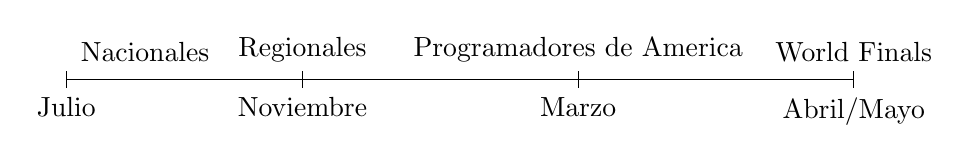
\begin{tikzpicture}
        \draw (1,0) -- (11,0);
        \foreach \x in {1,4,7.5,11}
            \draw (\x cm,3pt) -- (\x cm,-3pt);
            \draw (1,0) node[below=3pt] {Julio} node[above=3pt] {};
            \draw (2,0) node[below=3pt] {} node[above=3pt] {Nacionales};
            \draw (4,0) node[below=3pt] {Noviembre} node[above=3pt] {Regionales};
            \draw (7.5,0) node[below=3pt] {Marzo} node[above=3pt] {Programadores de America};
            \draw (11,0) node[below=3pt] {Abril/Mayo} node[above=3pt] {World Finals};
    \end{tikzpicture}
    \centering
    \begin{itemize}
        \item 3 personas
        \item 1 PC
        \item 10-14 problemas
        \item 5 horas
    \end{itemize}
\end{frame}

\section{Juez Online - Codeforces}
\begin{frame}{Codeforces}
    \centering
    
\includegraphics[height=2cm,keepaspectratio]{logos/codeforces-sponsored-by-ton.png}
    \begin{itemize}
        \item Juez online ruso.
        \item Funciona como test de caja negra, obtenemos una respuesta casi instantanea.
        \item Tiene rondas casi semanales, sistema de rating para usuarios similar al ELO.
        \item Usaremos este juez para todas las simulaciones.
    \end{itemize}
\end{frame}

\begin{frame}{Submit y respuestas}
    \centering
    Veamos algunos submits míos para conocer algunas respuestas.\\
    
\includegraphics[height=5cm]{img/shame.jpg}
\end{frame}

\section{Análisis de Complejidad}
\begin{frame}{Cantidad de operaciones}
    ¿Cuántas operaciones ``entran en tiempo''?
    \begin{itemize}
        \item Hasta $10^7$ : ¡Todo OK!
        \item Entre $10^7$ y hasta $10^9$: ``Tierra incógnita''. Puede cambiar mucho según el costo de las operaciones.
        \item Más de $10^9$: Casi con certeza total será demasiado lento.
    \end{itemize}
    Lo anterior asume:
        \begin{itemize}
            \item Hardware no extremadamente viejo.
            \item Límites de tiempo del orden de ``segundos'' (ni minutos, ni milésimas).
        \end{itemize}
\end{frame}

\begin{frame}{funcion O}
    \begin{itemize}
        \item La complejidad del tiempo de un algoritmo se anota como $O(\dots)$
        \item Los tres puntos pueden ser una función.
        \item La variable $n$ normalmente se refiere al tamaño del input.
    \end{itemize}
\end{frame}

\begin{frame}{Algunos ejemplos}
    \texttt{for (int i = 1; i <= n; i++) \{}\\
    \texttt{    //codigo}\\
    \texttt{\}}\\
    $O(n)$\\

    \hspace{1cm}\\

    \texttt{for (int i = 1; i <= n; i++) \{}\\
    \texttt{    for (int j = 1; j <= n; j++) \{}\\
    \texttt{        //codigo}\\
    \texttt{ \}\\ \}}\\
    $O(n^2)$
\end{frame}

\begin{frame}{Estimando eficiencia}
    \centering
    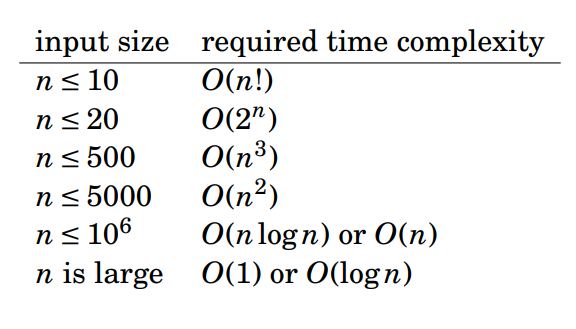
\includegraphics[height=7cm,keepaspectratio]{img/estimaciones.png}
\end{frame}


\section{Entrada y Salida}
\begin{frame}{¿Por qué conviene hacer eficiente la E/S?}
    %%\pause
    \begin{itemize}
    \item En problemas de complejidad lineal o similar, las operaciones de E/S pueden insumir un porcentaje importante del tiempo total de ejecución, que es lo que se mide en la mayoría de las competencias.
    \pause
    \invisible<1>{
        \item Aún si los tiempos elegidos por el jurado son generosos, y es posible con una solución esperada resolver el problema aún con mecanismos de E/S ineficientes, usar formas eficientes de hacer E/S nos permitirá siempre ``zafar'' con programas más lentos que si no lo hiciéramos así.
        \pause
        \invisible<1-2>{
          \item Existen diferencias \textbf{muy simples y pequeñas} en la forma de realizar E/S en los programas, que \textbf{generan grandes diferencias} en el tiempo total insumido por estas operaciones. Conocer estas diferencias es entonces obtener un beneficio relevante con muy poco esfuerzo.
        }
    }
    \end{itemize}
    
  \end{frame}
  
  
  \begin{frame}{Funciones printf y scanf}
  
    \begin{itemize}
        \item En C plano, la forma de E/S más utilizada son las funciones printf y scanf. Estas funciones \textbf{son eficientes}, y es la forma recomendada de realizar entrada salida en este lenguaje.
        \item Ejemplo:
        
  \texttt{\#include <stdio.h>}
  
  \texttt{int main() \{}
  
  \texttt{    \ \ \ int x,y;}
      
  \texttt{    \ \ \ scanf("\%d\%d", \&x, \&y);}
      
  \texttt{    \ \ \ printf("\%d\textbackslash n", x+y);}
      
  \texttt{\}}
    \end{itemize}
    
  \end{frame}
    
  \begin{frame}{Funciones printf y scanf}
  
    \begin{itemize}
        \item En C++, las mismas funciones scanf y printf siguen disponibles, y siguen siendo una opción eficiente para aquellos que estén acostumbrados o gusten de usarlas.
        \item Ejemplo:
        
  \texttt{\#include <cstdio>}
  
  \texttt{using namespace std;}
  
  \texttt{int main() \{}
  
  \texttt{    \ \ \ int x,y;}
      
  \texttt{    \ \ \ scanf("\%d\%d", \&x, \&y);}
      
  \texttt{    \ \ \ printf("\%d\textbackslash n", x+y);}
      
  \texttt{\}}
    \end{itemize}
    
  \end{frame}
  
  \begin{frame}{Streams cin y cout}
  
    \begin{itemize}
        \item La forma elegante de hacer E/S en C++ es mediante los streams cin y cout (Y análogos objetos fstream si hubiera que manipular archivos específicos en alguna competencia).
        \item Ejemplo:
        
  \texttt{\#include <cstdio>}
  
  \texttt{using namespace std;}
  
  \texttt{int main() \{}
  
  \texttt{    \ \ \ int x,y;}
      
  \texttt{    \ \ \ cin >{}> x >{}> y;}
      
  \texttt{    \ \ \ cout <{}< x+y <{}< endl;}
      
  \texttt{\}}
    \end{itemize}
    
  \end{frame}
  
  \begin{frame}{Por defecto en casos usuales, cin y cout son lentos}
  
    \begin{itemize}
        \item La eficiencia relativa de cin y cout vs scanf y printf dependerá del compilador y arquitectura en cuestión.
        \item Dicho esto, en la mayoría de los compiladores y sistemas usuales utilizados en competencia, cin y cout son por defecto \textbf{mucho} más lentos que scanf y printf.
        \item Veremos algunos trucos para que cin y cout funcionen más rápido. Con ellos, en algunos sistemas comunes funcionan más rápido que printf y scanf, pero la diferencia es muy pequeña.
        \item En otras palabras, aplicando los trucos que veremos a continuación, da igual usar cin y cout o printf y scanf, ambas son eficientes.
    \end{itemize}
    
  \end{frame}
  
  \begin{frame}{Primera observación: endl}
  
    \begin{itemize}
        \item El valor ``endl'' no es solo un fin de línea, sino que además ordena que se realice un \textbf{flush del buffer}.
        \item De esta forma, imprimir muchas líneas cortas (un solo entero, un solo valor Y/N, etc) realiza muchas llamadas a escribir directamente al sistema operativo, para escribir unos poquitos bytes en cada una.
        \item \textbf{Solución:} utilizar \texttt{\textbackslash n} en su lugar. Esto es un sencillo caracter de fin de línea, que no ejecuta un flush del buffer.
        \item Ejemplo:
        
  \texttt{\#include <cstdio>}
  
  \texttt{using namespace std;}
  
  \texttt{int main() \{}
  
  \texttt{    \ \ \ int x,y;}
      
  \texttt{    \ \ \ cin >{}> x >{}> y;}
      
  \texttt{    \ \ \ cout <{}< x+y <{}< \textbf{"\textbackslash n"};}
      
  \texttt{\}}
    \end{itemize}
    
  \end{frame}
  
  \begin{frame}{Segunda observación: sincronización con stdio}
  
    \begin{itemize}
        \item Por defecto, cin y cout están sincronizados con todas las funciones de stdio (notablemente, scanf y printf). Esto significa que si usamos ambos métodos, las cosas se leen y escriben en el orden correcto.
        \item En varios de los compiladores usuales esto vuelve a cin/cout \textbf{mucho} más lentos, y si solamente usamos cin y cout pero \textbf{nunca scanf y printf}, no lo necesitamos.
        \item \textbf{Solución:} utilizar \texttt{ios::sync\_with\_stdio(false)} al iniciar el programa, para desactivar esta sincronización. Notar que si hacemos esto, \textbf{ya no podemos usar printf ni scanf} (ni ninguna función de stdio) sin tener resultados imprevisibles.
        \item Desactivar la sincronización también puede tener efectos al utilizar más de un thread. Esto no nos importa en ICPC.
    \end{itemize}
    
  \end{frame}
  
  \begin{frame}{Segunda observación: sincronización (ejemplo)}
  
  Esta optimización tiene efectos muy notorios, típicamente reduce el tiempo de ejecución a la mitad en varios jueces online comunes.
  
  Ejemplo:
        
  \texttt{\#include <cstdio>}
  
  \texttt{using namespace std;}
  
  \texttt{int main() \{}
  
  \textbf{\texttt{    \ \ \ ios::sync\_with\_stdio(false);}}
  
  \texttt{    \ \ \ int x,y;}
      
  \texttt{    \ \ \ cin >{}> x >{}> y;}
      
  \texttt{    \ \ \ cout <{}< x+y <{}< "\textbackslash n";}
      
  \texttt{\}}
  
  \end{frame}
  
  
  \begin{frame}{Tercera observación: dependencia entre cin y cout}
  
    \begin{itemize}
        \item Por defecto, cin está \textit{atado} a cout, lo cual significa que siempre antes de leer de cin, se fuerza un flush de cout. Esto hace que programas interactivos funcionen como se espera.
        \item Cuando solo se hacen unas pocas escrituras con el resultado al final de toda la ejecución, esto no tiene un efecto tan grande.
        \item Si por cada línea que leemos escribimos una en la salida, este comportamiento fuerza un flush en cada línea, como hacía endl.
        \item \textbf{Solución:} utilizar \texttt{cin.tie(nullptr)} al iniciar el programa, para desactivar esta dependencia. Notar que si hacemos esto, tendremos que realizar flush de cout manualmente si queremos un programa interactivo.
    \end{itemize}
    
  \end{frame}
  
  \begin{frame}{Tercera observación: dependencia (ejemplo)}
        
  \texttt{\#include <cstdio>}
  
  \texttt{using namespace std;}
  
  \texttt{int main() \{}
  
  \texttt{    \ \ \ ios::sync\_with\_stdio(false);}
  
  \textbf{\texttt{    \ \ \ cin.tie(nullptr);}}
  
  \texttt{    \ \ \ int x,y;}
      
  \texttt{    \ \ \ cin >{}> x >{}> y;}
      
  \texttt{    \ \ \ cout <{}< x+y <{}< "\textbackslash n";}
      
  \texttt{\}}
  
  \end{frame}
  
  \begin{frame}{Ejemplo final con las 3 técnicas}
        
        \begin{itemize}
             \item Eliminar sincronización con stdio
             \item Eliminar dependencia entre cin y cout
             \item No utilizar endl
        \end{itemize}
        
  \texttt{\#include <cstdio>}
  
  \texttt{using namespace std;}
  
  \texttt{int main() \{}
  
  \textbf{\texttt{    \ \ \ ios::sync\_with\_stdio(false);}}
  
  \textbf{\texttt{    \ \ \ cin.tie(nullptr);}}
  
  \texttt{    \ \ \ int x,y;}
      
  \texttt{    \ \ \ cin >{}> x >{}> y;}
      
  \texttt{    \ \ \ cout <{}< x+y <{}< \textbf{"\textbackslash n"};}
      
  \texttt{\}}
  
  \end{frame}
  
\section{Estructuras fundamentales}
    
\begin{frame}{Vector}
    \begin{itemize}
        \item vector$<$int$>$ en C++, con push\_back y pop\_back
        \item ArrayList$<$Integer$>$ en Java, con .add y .remove(list.size()-1)
        \item list en Python (listas usuales como [1,2,3]), con .append y .pop
        \item acceso con lista[i] o lista.get(i)
        \item Sirven como \textbf{pila}
        \item Las operaciones anteriores son $O(1)$ (amortizado)
    \end{itemize}
\end{frame}

\begin{frame}{Queue}
    \begin{itemize}
        \item queue$<$int$>$ en C++, con push, front y pop
        \item ArrayDeque$<$Integer$>$ en Java, con .add, .getFirst y .remove
        \item collections.deque en Python, con .append, deque[0] y .popleft
        \item Sirven como \textbf{cola}
        \item Las operaciones anteriores son $O(1)$ (amortizado)
    \end{itemize}
\end{frame}

\begin{frame}{Deque}
    \begin{itemize}
        \item deque$<$int$>$ en C++, con push\_front, push\_back, pop\_front y pop\_back
        \item ArrayDeque$<$Integer$>$ en Java, con .addFirst, .addLast, .removeFirst y .removeLast
        \item collections.deque en Python, con .appendleft, .append, .popleft y .pop
        \item acceso con lista[i] (\textbf{no se puede en java!!})
        \item Sirven como \textbf{cola de dos puntas}
        \item Las operaciones anteriores son $O(1)$ (amortizado)
    \end{itemize}
\end{frame}

\begin{frame}{HashSet}
    \begin{itemize}
        \item unordered\_set$<$int$>$ en C++
        \item HashSet$<$Integer$>$ en Java
        \item set en Python
        \item Permiten insertar, borrar y consultar pertenencia en $O(1)$
    \end{itemize}
\end{frame}

\begin{frame}{HashMap}
    \begin{itemize}
        \item unordered\_map$<$int,int$>$ en C++
        \item HashMap$<$Integer,Integer$>$ en Java
        \item dict en Python
        \item Permiten insertar, borrar y consultar pertenencia en $O(1)$
        \item Son casi iguales a los HashSet, pero guardan un \textbf{valor asociado} a cada elemento
    \end{itemize}
\end{frame}

\begin{frame}{Set}
    \begin{itemize}
        \item set$<$int$>$ en C++
        \item TreeSet$<$Integer$>$ en Java (googlear docs de NavigableSet)
        \item En Python no hay. ¡Ojo! \\ collections.OrderedDict \textbf{es otra cosa} (LinkedHashMap de Java)
        \item Permiten insertar, borrar, consultar pertenencia y hacer \texttt{s.lower\_bound} o \texttt{s.upper\_bound} en $O(\lg N)$
    \end{itemize}
\end{frame}

\begin{frame}{TreeMap}
    \begin{itemize}
        \item map$<$int,int$>$ en C++
        \item TreeMap$<$Integer,Integer$>$ en Java (googlear docs de NavigableMap)
        \item No confundir ``collections.OrderedDict'' \textbf{(que no es..)}
        \item Permiten insertar, borrar, consultar pertenencia y hacer \texttt{m.lower\_bound} o \texttt{m.upper\_bound} en $O(\lg N)$
        \item Son casi iguales a los TreeSet, pero guardan un \textbf{valor asociado} a cada elemento
    \end{itemize}
\end{frame}

\section{Funciones clave (C++)}

\begin{frame}{Funciones clave (C++)}
    \begin{itemize}
        \item \texttt{sort} (algorithm) [begin, end]
        \item \texttt{lower\_bound , upper\_bound, equal\_range} (algorithm) [begin, end, val]. \textbf{¡¡NO USAR CON SET Y MAP!!}
        \item \texttt{find} (algorithm) [begin, end, val]
        \item \texttt{max\_element, min\_element} (algorithm) [begin, end]
    \end{itemize}
\end{frame}

\section{Overflow}
\begin{frame}{Overflow}
    \begin{itemize}
        \item Si uno no presta atención, es \textbf{extremadamente común} tener errores por culpa del overflow de enteros.
        \item Es importante acostumbrarse a \textbf{siempre} revisar las cotas de todas las entradas, y calcular los posibles valores máximos de los números que maneja el programa. Suele ser multiplicar cotas de la entrada.
        \item Ante la duda preferir tipos de 64 bits (long long en C++, long en Java) a tipos de 32 bits (int).
        \item Ojo con \\ \texttt{long long mask = 1 << 33;} \\  que está mal. Debería ser \\ \texttt{long long mask = 1LL << 33;}
        \item int: hasta $2^{31}-1 = 2.147.483.647$. Algo más de dos mil millones.
        \item long long: hasta $2^{63}-1$. Más de $10^{18}$, pero menos que $10^{19}$.
    \end{itemize}
\end{frame}


\begin{frame}{Consultas}
Pueden consultarme durante esta semana, o me pueden enviar un mail a:
        \begin{itemize}
            \item \href{mailto:mramos@frsf.utn.edu.ar}{mramos@frsf.utn.edu.ar}
        \end{itemize}
        %\bibliography{ref}
\end{frame}


\end{document}